\chapter*{说明}

\begin{center}

    \arm{\ait {\Large اُطْلُبُوْا العِلْمَ وَلَوْ في الصِّينِ.}}
    
    ~\\

    \emph{求知,哪怕在中国。}
\end{center}
\vfill

\begin{wrapfigure}{r}{0.3\textwidth}
    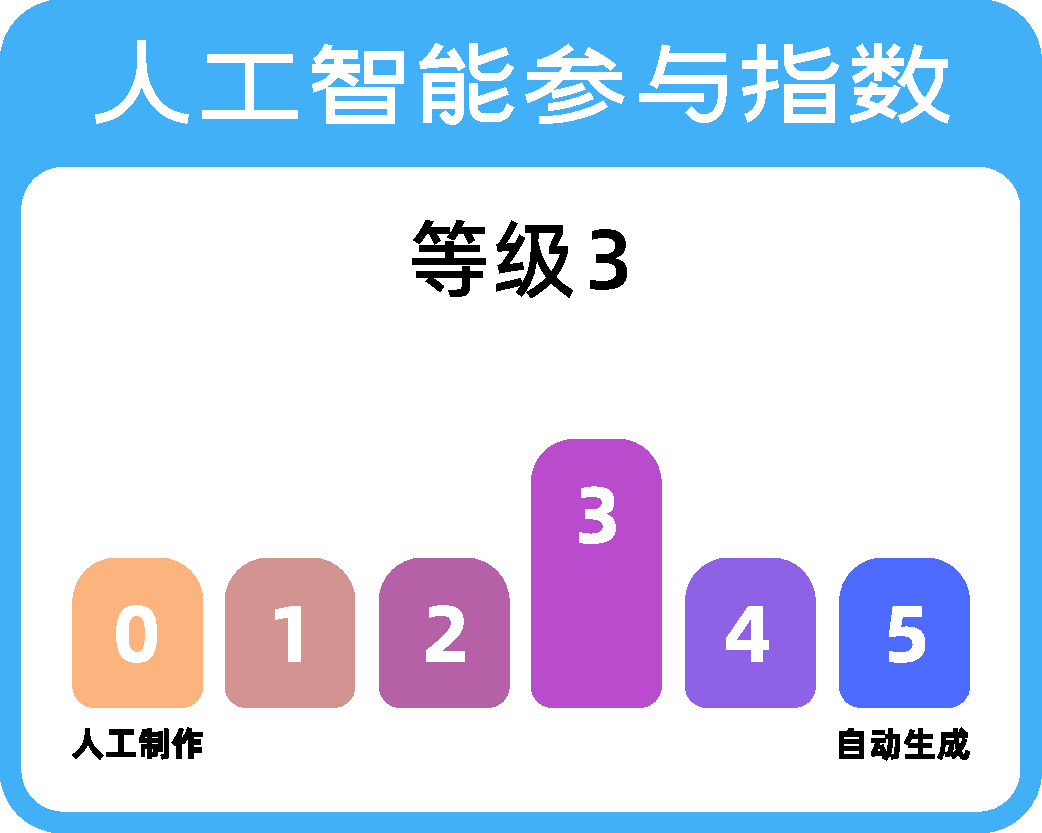
\includegraphics[width=0.3\textwidth]{img/iiia.pdf}
\end{wrapfigure}

作为一个跟着课程进度现学的初学者,阿语键盘用起来实在是太痛苦了。一方面,键位记起来很难;另一方面,它默认把发音符号藏在了辅助键下,总是需要按组合按键才能打出,一些符号(比如 \arm{ ٍ} 字符)的组合键还会跟软件本身的快捷键冲突。所以,本笔记的阿语部分借助GitHub Copilot生成了不少。这玩意很好用,甚至能猜到接下来的例句(不过发音符号有时会标错)。

我对照课程内容,人工审核了AI生成的所有内容,但由于毕竟是新接触一套书写系统,难免有拼写疏漏。我会随时发现随时修正。

AI也帮我解决了许多排版和字体渲染上的问题。

\subsection*{格式约定}

\lecon{$\cdot$} 这样的格式代表对应课程的序号。

\begin{attention}
    这样的格式代表老师在课上强调的知识点。
\end{attention}

\begin{note}
    这样的格式代表我自己的感悟。
\end{note}